% DPF 09 talk on strangeness in nucleon
\documentclass[10pt]{beamer}
\usepackage{amsmath}
\usepackage{mathtools}
\usepackage{multimedia}
\usepackage{hyperref}
\usefonttheme{professionalfonts} % using non standard fonts for beamer
\usefonttheme{serif} % default family is serif
%\documentclass[12pt]{beamerthemeSam.sty}
\usepackage{epsf}
%\usepackage{pstricks}
%\usepackage[orientation=portrait,size=A4]{beamerposter}
\geometry{paperwidth=160mm,paperheight=120mm}
%DT favorite definitions
\def\LL{\left\langle}	% left angle bracket
\def\RR{\right\rangle}	% right angle bracket
\def\LP{\left(}		% left parenthesis
\def\RP{\right)}	% right parenthesis
\def\LB{\left\{}	% left curly bracket
\def\RB{\right\}}	% right curly bracket
\def\PAR#1#2{ {{\partial #1}\over{\partial #2}} }
\def\PARTWO#1#2{ {{\partial^2 #1}\over{\partial #2}^2} }
\def\PARTWOMIX#1#2#3{ {{\partial^2 #1}\over{\partial #2 \partial #3}} }

\def\rightpartial{{\overrightarrow\partial}}
\def\leftpartial{{\overleftarrow\partial}}
\def\diffpartial{\buildrel\leftrightarrow\over\partial}

\def\BS{\bigskip}
\def\BC{\begin{center}}
\def\EC{\end{center}}
\def\BI{\begin{itemize}}
\def\EI{\end{itemize}}
\def\BE{\begin{displaymath}}
\def\EE{\end{displaymath}}
\def\BEA{\begin{eqnarray*}}
\def\EEA{\end{eqnarray*}}
\def\BNEA{\begin{eqnarray}}
\def\ENEA{\end{eqnarray}}
\def\EL{\nonumber\\}


\newcommand{\map}[1]{\frame{\frametitle{\textbf{Course map}}
\centerline{\includegraphics[height=0.86\paperheight]{../../map/#1.png}}}}
\newcommand{\wmap}[1]{\frame{\frametitle{\textbf{Course map}}
\centerline{\includegraphics[width=0.96\paperwidth]{../../map/#1.png}}}}

\newcommand{\etal}{{\it et al.}}
\newcommand{\gbeta}{6/g^2}
\newcommand{\la}[1]{\label{#1}}
\newcommand{\ie}{{\em i.e.\ }}
\newcommand{\eg}{{\em e.\,g.\ }}
\newcommand{\cf}{cf.\ }
\newcommand{\etc}{etc.\ }
\newcommand{\atantwo}{{\rm atan2}}
\newcommand{\Tr}{{\rm Tr}}
\newcommand{\dt}{\Delta t}
\newcommand{\op}{{\cal O}}
\newcommand{\msbar}{{\overline{\rm MS}}}
\def\chpt{\raise0.4ex\hbox{$\chi$}PT}
\def\schpt{S\raise0.4ex\hbox{$\chi$}PT}
\def\MeV{{\rm Me\!V}}
\def\GeV{{\rm Ge\!V}}

%AB: my color definitions
%\definecolor{mygarnet}{rgb}{0.445,0.184,0.215}
%\definecolor{mygold}{rgb}{0.848,0.848,0.098}
%\definecolor{myg2g}{rgb}{0.647,0.316,0.157}
\definecolor{A}{rgb}{1.0,0.3,0.3}
\definecolor{B}{rgb}{0.0,1.0,0.0}
\definecolor{C}{rgb}{1.0,1.0,0.0}
\definecolor{D}{rgb}{0.5,0.5,1.0}
\definecolor{E}{rgb}{0.7,0.7,0.7}
\definecolor{abtitlecolor}{rgb}{1.0,1.0,1.0}
\definecolor{absecondarycolor}{rgb}{0.0,0.416,0.804}
\definecolor{abprimarycolor}{rgb}{1.0,0.686,0.0}
\definecolor{Red}           {cmyk}{0,1,1,0}
\definecolor{Grey}          {cmyk}{.7,.7,.7,0}
\definecolor{Blue}          {cmyk}{1,1,0,0}
\definecolor{Green}         {cmyk}{1,0,1,0}
\definecolor{Brown}         {cmyk}{0,0.81,1,0.60}
\definecolor{Silver}        {rgb}{0.95,0.9,1.0}
\definecolor{Sky}           {rgb}{0.07,0.0,0.2}
\definecolor{Darkbrown}     {rgb}{0.4,0.3,0.2}
\definecolor{40Gray}        {rgb}{0.4,0.4,0.5}
\usetheme{Madrid}


\setbeamercolor{normal text}{fg=Silver,bg=Sky}

%AB: redefinition of beamer colors
%\setbeamercolor{palette tertiary}{fg=white,bg=mygarnet}
%\setbeamercolor{palette secondary}{fg=white,bg=myg2g}
%\setbeamercolor{palette primary}{fg=black,bg=mygold}
\setbeamercolor{title}{fg=abtitlecolor}
\setbeamercolor{frametitle}{fg=abtitlecolor}
\setbeamercolor{palette tertiary}{fg=white,bg=Darkbrown}
\setbeamercolor{palette secondary}{fg=white,bg=absecondarycolor}
\setbeamercolor{palette primary}{fg=white,bg=40Gray}
\setbeamercolor{structure}{fg=abtitlecolor}

\setbeamerfont{section in toc}{series=\bfseries}

%AB: remove navigation icons
\beamertemplatenavigationsymbolsempty
\title[Introduction to Astronomy]{
  \textbf {What's out there... \\ ... how we learn about it ... \\ ... and why it's awesome. \\}
%\centerline{}
%\centering
%\vspace{-0.0in}
%\includegraphics[width=0.3\textwidth]{propvalues_0093.pdf}
%\vspace{-0.3in}\\
%\label{intrograph}
}

\author [Astronomy 101]{Astronomy 101\\Syracuse University, Fall 2018\\Walter Freeman}

\date{\today}

\begin{document}

\frame{\titlepage}

\frame{\frametitle{\textbf{Welcome!}}
\large

The size and age of the Cosmos are beyond ordinary human understanding. 
Lost somewhere between immensity and eternity is our tiny planetary home. 
In a cosmic perspective, most human concerns seem insignificant, even petty. 
And yet our species is young and curious and brave and shows much promise. 
In the last few millennia we have made the most astonishing and unexpected discoveries about the Cosmos and our place within it, 
explorations that are exhilarating to consider. 
They remind us that humans have evolved to wonder, that understanding is a joy, 
that knowledge is prerequisite to survival. 
I believe our future depends powerfully on how well we understand this Cosmos in which we float like a mote of dust in the morning sky.

\bigskip
\bigskip

\begin{flushright}--Carl Sagan, from {\it Cosmos}\end{flushright}
}

\frame{\frametitle{\textbf{Welcome!}}
\Large
Today:

\begin{itemize}
\item{Who we are}
\item{Who you are}
\item{What this class will be}
\pause
\item{What the Universe is, too}

\small \it (and how we measure it)

\end{itemize}
}

\frame{\frametitle{\textbf{Introduction}}
\Large
Course website: \url{https://walterfreeman.github.io/ast101/}

\BI
\item{Professor: Walter Freeman}
\item{Lead TA: Scott Bassler}
\item{Other TA's...}
\item{Undergraduate coaches...}
\EI

\bigskip
\bigskip

\begin{tabular}{ll}
My email: & \href{mailto:wafreema@syr.edu}{wafreema@syr.edu} \\
Sumar's email: & \href{mailto:skundu@syr.edu}skundu@syr.edu \\
\end{tabular}
}
\frame{\frametitle{\textbf{Introduction}}
\Large
Course website: \url{https://walterfreeman.github.io/ast101/}
\color{gray}
\BI
\color{gray}
\item{Professor: Walter Freeman}
\item{Lead TA: Sumar Kundu}
\item{Other TA's}
\item{Undergraduate coaches}
\EI

\bigskip
\bigskip

\begin{tabular}{ll}
My email: & \color{white}\href{mailto:wafreema@syr.edu}{wafreema@syr.edu} \\
Sumar's email: & \href{mailto:skundu@syr.edu}skundu@syr.edu \\
\end{tabular}
}


\frame{\frametitle{\textbf{Clickers}}
\Large 
You all should have gotten a clicker with your textbook from the bookstore.

\pause
\bigskip
\bigskip
\bigskip

... wait, you didn't?

\begin{columns}

\begin{column}{0.5\textwidth}
\end{column}
\pause
\begin{column}{0.5\textwidth}
...I guess we have some extras...

\pause

\bigskip

\includegraphics[width=0.6\textwidth]{trollface.png}

\pause

\end{column}
\end{columns}
\bigskip
\bigskip
\bigskip


We're using an extremely high-tech, state-of-the-art clicker system in this class.
Make sure you get one, and bring it to class every day.

}

\frame{\frametitle{\textbf{Who are you?}}
\Large
What academic year are you?
\bigskip

\Huge

\color{A}A: Freshman \\
\color{B}B: Sophomore \\
\color{C}C: Junior \\
\color{D}D: Senior \\
\color{E}E: Graduate student / non-degree

}

\frame{\frametitle{\textbf{Who are you?}}
\Large
What's your primary field of study?

\bigskip

\Huge

\color{A}A: Science / engineering \\
\color{B}B: Social sciences / Maxwell / international relations\\
\color{C}C: Management / business / accounting\\
\color{D}D: SUNY ESF \\
\color{E}E: None of these

\Large

\bigskip
\bigskip
}

\frame{\frametitle{\textbf{Who are you?}}
\Large
What's your primary field of study?

\bigskip
\Huge

\color{A}A: Visual / performing arts \\ 
\color{B}B: Liberal arts / humanities\\
\color{C}C: Communication / Newhouse \\
\color{D}D: The iSchool \\ 
\color{E}E: Something else 

}

\frame{\frametitle{\textbf{Who are you?}}
\Large
What's your primary field of study?

\bigskip
\Huge

\color{white}A: Visual / performing arts \\ 
\color{white}B: Liberal arts / humanities \\
\color{white}C: Communication / Newhouse \\
\color{blue}D: The iSchool \\ 
\color{blue}E: Something else 

}

\frame{\frametitle{\textbf{Someone threw a gauntlet at you...}}

\large
``With more knowledge comes deeper, more wonderful mystery... 
with pleasure and confidence we turn over each new stone to find 
unimagined strangeness leading on to more wonderful questions and mysteries--certainly
a grand adventure!

\bigskip

Our poets 
do not write about [this]; our artists do not try to portray [it]. I don't know why. 
{\bf Is nobody inspired by our present picture of the universe?} [Science] remains unsung
by singers, so you are reduced to hearing not a song or poem, but an evening lecture about it.
Is no one inspired by our present picture of the universe? {\bf This is not yet a 
scientific age.}''

\bigskip
\bigskip

\begin{flushright}--Richard Feynman, from {\it The Value of Science} (1955)
\end{flushright}
}

\frame{\frametitle{\textbf{Do you agree with Feynman?}}
\Large
... are we not yet living in a ``scientific age''? Were we in 1955?

\bigskip


\color{A}A: No, we don't live in a scientific age \\ 
\color{B}B: We didn't then, but we do now \\
\color{C}C: We did then, and we still do! \\
\color{D}D: What a silly question! 

\pause

My answer comes in three parts...
}

\frame{\frametitle{\textbf{Our poets and writers have (always) been busy...}}
\includegraphics[width=1.0\textwidth]{collage.jpg}
}

\frame{\frametitle{\textbf The source of all wisdom: tumblr.}
\begin{columns}
\column{0.5\textwidth}
\includegraphics[width=\textwidth]{sad-thing.png}
\pause
\column{0.5\textwidth}
\includegraphics[width=\textwidth]{awesome-thing.png}

\bigskip
\begin{center}
\it \scriptsize (source: thebaconsandwichofregret.tumblr.com)
\end{center}
\end{columns}
}

\frame{\frametitle{\textbf{The eclipse of 2017}}

\BC
\includegraphics[width=0.8\textwidth]{lisk-corona.jpg}
\small

\it(by Keith Lisk, shot in Paducah, KY: \url{https://www.dpreview.com/forums/post/60016117})
\EC
}
\frame{\frametitle{\textbf{The eclipse of 2017}}

\BC
\includegraphics[width=0.8\textwidth]{viralclimber1.jpeg}
\tiny

\it(photographers Andrew Studer and Ted Hesser; climbers Tommy Smith and Martina Tibell; Smith Rock State Park, OR)
\EC
\small
\BS
\url{https://www.dpreview.com/articles/5501288570/how-the-viral-climber-eclipse-photo-and-video-were-shot}

\url{https://youtu.be/H6rxml7TRf0}
}



\frame{\frametitle{\textbf{Astronomy's broader impact on human thought}}
\Large
Astronomy has been inspiring art, philosophy, music, and literature since those things
have existed. 

\bigskip
\bigskip

Why is the fourth planet named Mars?

\bigskip
\bigskip
\bigskip

We're going to spend much of our class looking up ... but we'll spend a bit of time
looking back down, too, to see how astronomy has influenced so many fields of human endeavor.
}

\frame{\frametitle{\textbf{Course organization: four units}}
\Large
\begin{enumerate}
\item{Naked-eye astronomy}
\item{Astromechanics}
\item{The science of light}
\item{Humanity and the cosmos}
\end{enumerate}
}

\frame{\frametitle{\textbf{Naked-eye astronomy}}
\Large
\begin{columns}
  \begin{column}{0.5\textwidth}
  \BI
    \item{What can we see from Earth?}
    \item{What changes do we see in the sky?}
    \item{How are they explained by Earth's motion?}
  \EI
  \end{column}
  \begin{column}{0.5\textwidth}
  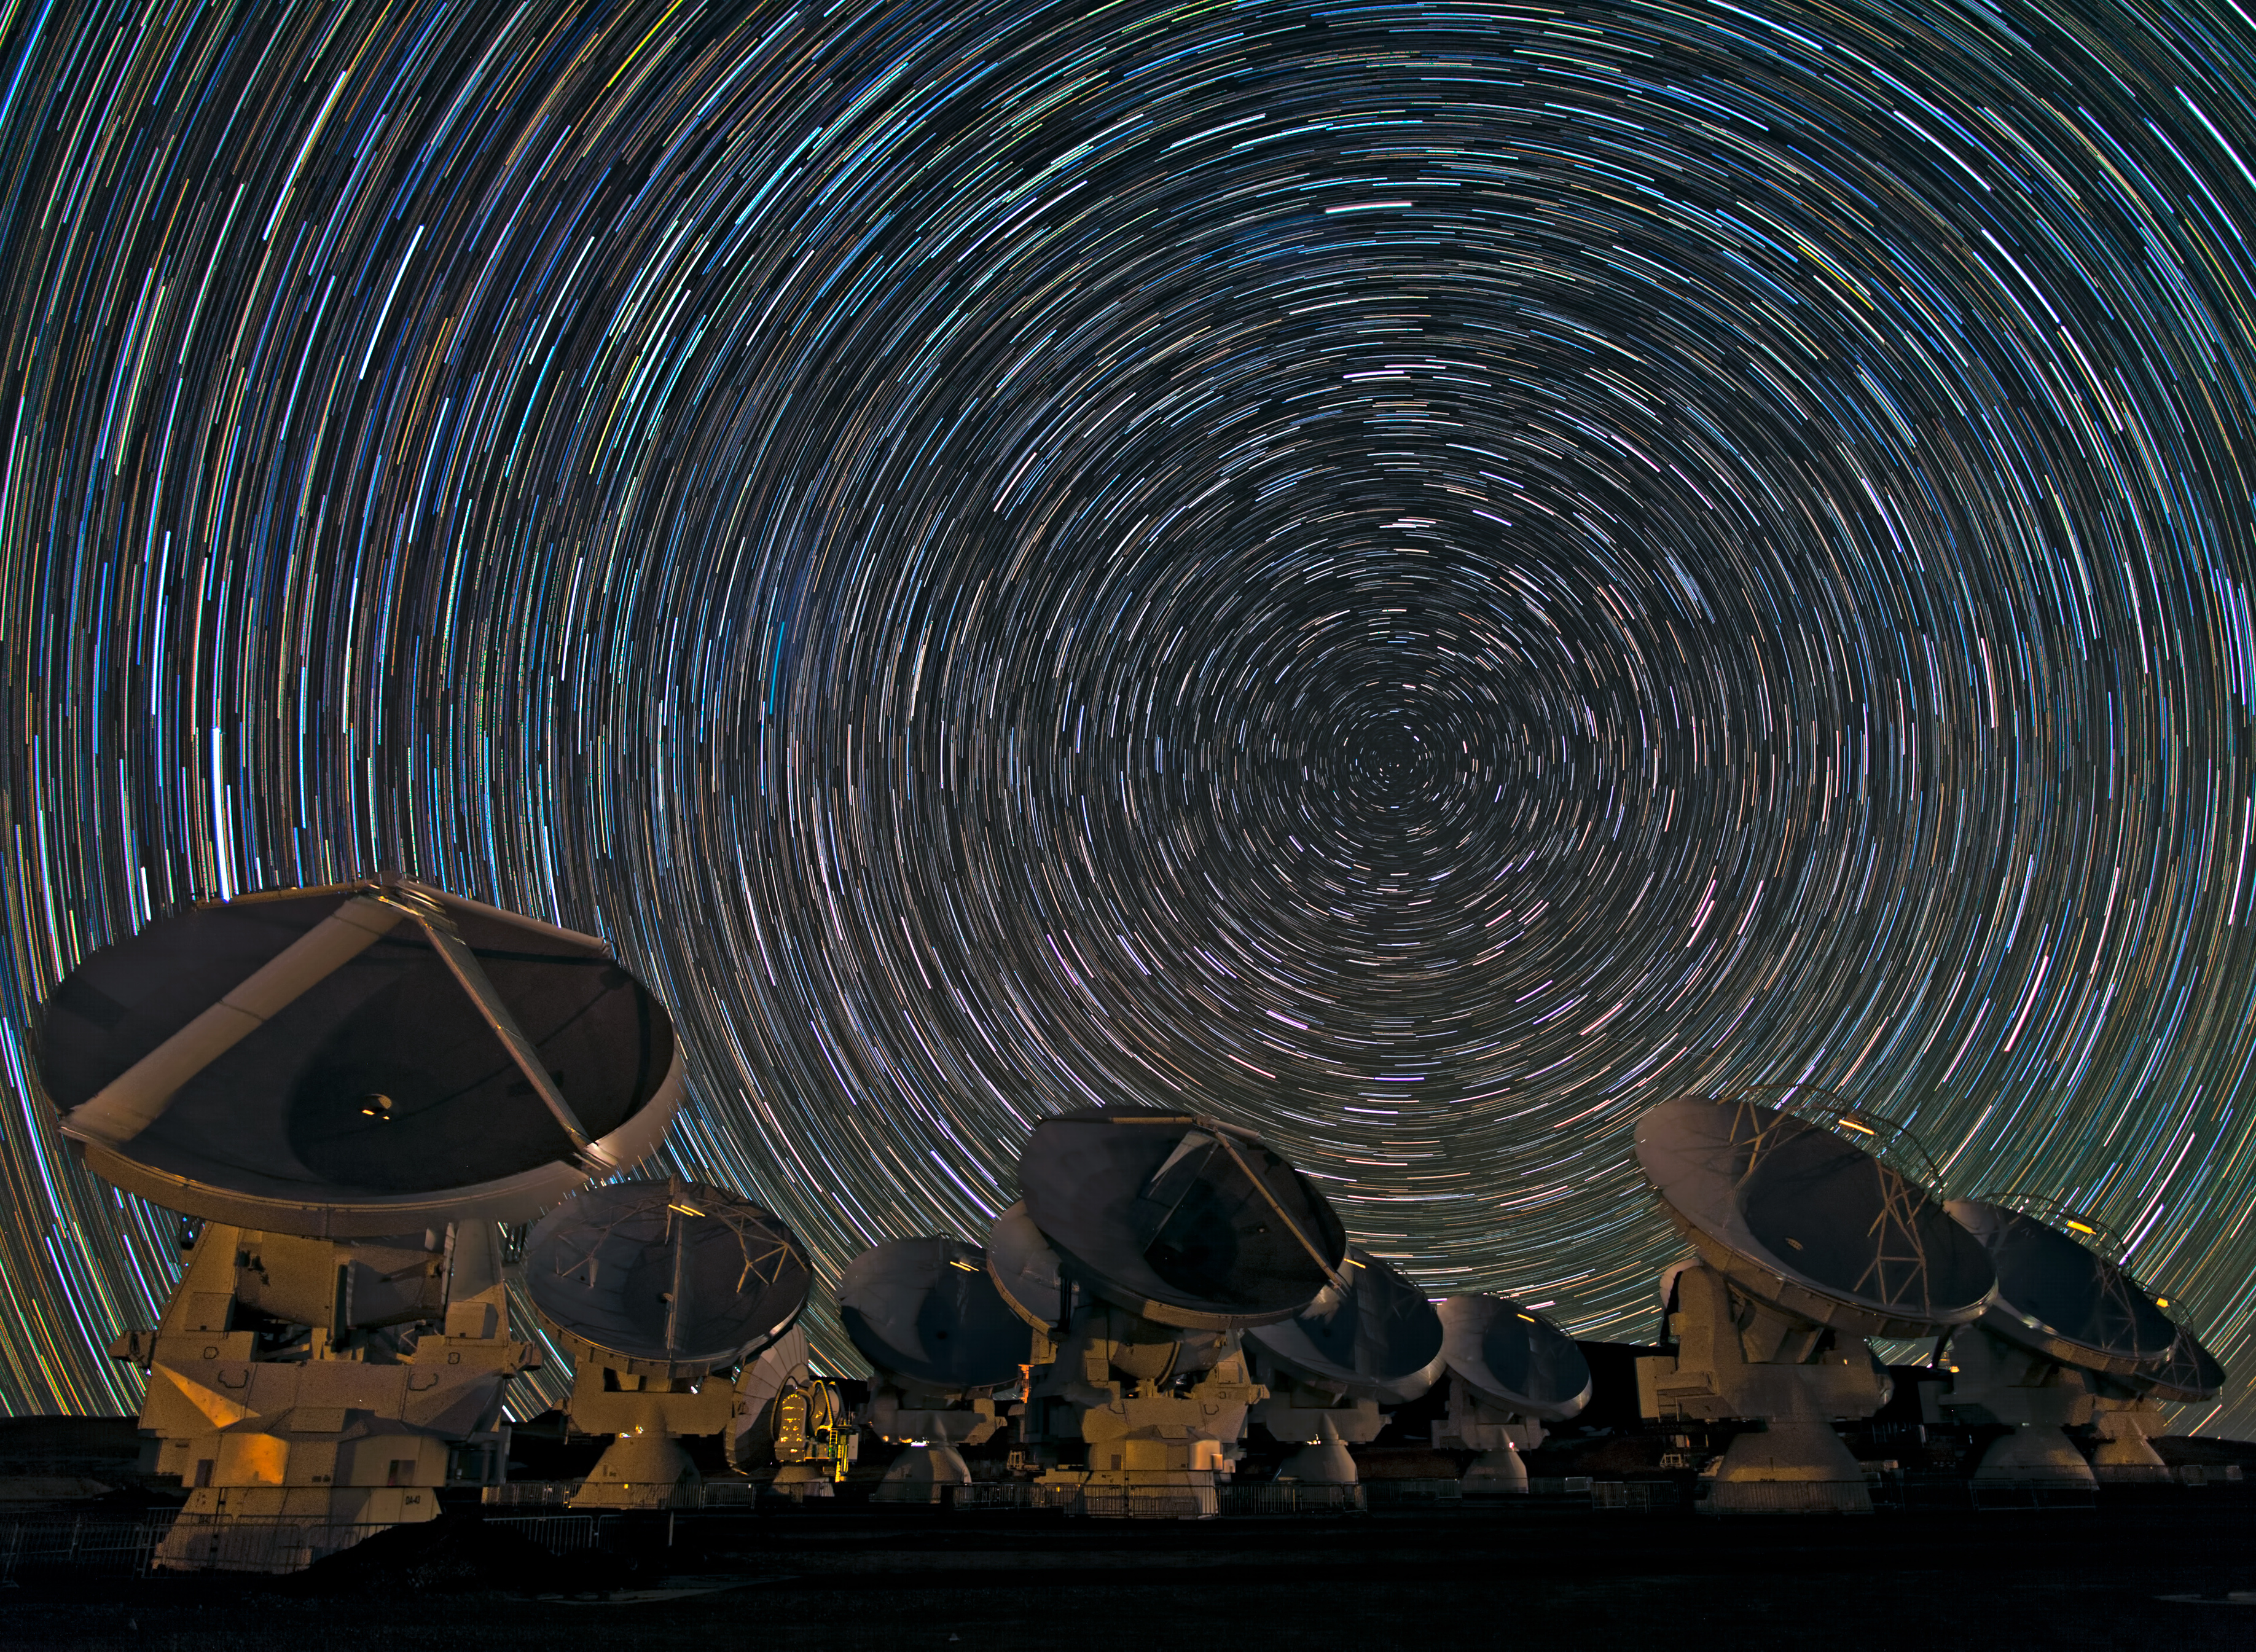
\includegraphics[width=1.0\textwidth]{alma-star-trails.jpg}
\end{column}
\end{columns}
}

\frame{\frametitle{\textbf{Astromechanics}}
\Large
\begin{columns}
  \begin{column}{0.5\textwidth}
  \BI
\item{How does scientific thought work?}
\medskip
\item{How do we know the planets orbit the Sun?} 
\medskip
\item{What do the motions of the planets really look like?}
\medskip
\item{How do the laws of physics cause them to move this way?}
\medskip
  \EI
  \end{column}
  \begin{column}{0.5\textwidth}
  \includegraphics[width=1.0\textwidth]{kep6.png}
\end{column}
\end{columns}
}

\frame{\frametitle{\textbf{Light and the electromagnetic spectrum}}
\Large
\begin{columns}
  \begin{column}{0.5\textwidth}
  \BI
\item{What is light?}
\medskip
\item {How does a telescope work?}
\medskip
\item{Where does light come from, and what does it do?}
\medskip
\item{How do we use light to study the sky?}
\medskip
\item{What has this taught us about the Sun?}
  \EI
  \end{column}
  \begin{column}{0.5\textwidth}
  \includegraphics[width=1.0\textwidth]{blackbody-spectrum.png}
  \end{column}
\end{columns}
}

\frame{\frametitle{\textbf{Humanity and the cosmos}}
\Large
  \BI
\item{What are the past and present of spaceflight?}
\item{... what might its future be in our lifetimes and beyond...}
\item{... and where else in the Universe might we find life, and what might it look like?}
  \EI
\begin{center}  \includegraphics[width=0.7\textwidth]{moonshorty_apollo17_1498.jpg}
\end{center}
}

\frame{\frametitle{\textbf{Course components: the labs}}
\Large
\BI
\item{Labs start on the {\bf second week of class}}
\item{ {\bf Prelabs:} Every lab has a prelab. You {\it must} complete the prelab and bring it with you to lab, or you won't be able to do that lab.}
\item{Take-home labs assigned next week, due at the end of the term}
\item{Labs meet in Holden Observatory, led by TA's}
\EI
}

\frame{\frametitle{\textbf{Course components: homework}}
\large
What kind of homework/classwork do you have in your philosophy class?

\pause\bigskip

... you're going to be writing a few papers, and doing a final creative project (which might be another paper),
in this class, too. These papers and project will focus on connections between the science of astronomy and 
other disciplines in the humanities.

\pause\bigskip

Your other homework:

\BI
\item Read the textbook
\item Make sure you understand the thought process behind the {\it Lecture Tutorials} questions
\EI
}





\frame{\frametitle{\textbf{Course components: other things}}
\Large
\BI
\item{``Lectures''}
\pause
\item{In-class tutorials -- bring your books!}
\pause
\item{Exams}
\pause
\item{Lots of details in the syllabus}
\EI
}

\frame{\frametitle{\textbf{I'm here to help you!}}
\Large
My full-time job is to help you all (and my other students). This is your class, not mine.

\bigskip
This means:
\BI
\large
\item{Interrupt me any time in class if you have a question}
\item{Yell at me if you have a question and I don't see your hand}
\item{Email me and ask for help: wafreema@syr.edu}
\item Send a message to the Slack channel, or private message me on Slack
\item{Come to office hours: Wednesdays, 3-5 PM, and Fridays, 9:30-11:30 AM (maybe not this Friday, though)}
\item{Come bang on my office door (room 215) -- I'll often be around}
\item{If you have questions you'd like addressed (``ask the physicist!''), or course suggestions, please send them to me (and get extra credit, if they're good!)}
\EI
}

\frame{\frametitle{\textbf{The cosmic perspective: measuring distance}}
\Large
\begin{center} \color{Red}``Baltimore is about five hours away.''\end{center}

Does this statement make sense as a way to describe the distance to Baltimore?

\bigskip
\bigskip

\color{A}A: Yes \\ 
\color{B}B: No  \\
\color{C}C: Yes, if I give you some other information...

\bigskip
\bigskip

}

\frame{\frametitle{\textbf{The cosmic perspective: measuring distance}}
\Large
\begin{center} \color{Red}``China is about 1/15 of a second away.''\end{center}

\pause

\normalsize (This is something anyone who's tried to play a video game with someone 
across the ocean knows about!)

\bigskip
\bigskip

\large
\pause
$\rightarrow$ We can measure long distances by {\it how long it takes light to get there!}

... if China is one-fifteenth of a light-second away, then a {\it light-year} has to be
a pretty long way...
}

\frame{\frametitle{\textbf{Three measures of distance...}}
\Large
Inside the Solar System, it's also useful to measure distances with a different yardstick:
the distance to the Sun. This is called an {\color{Red}astronomical unit}, or AU.

\bigskip

We have:

\bigskip

\begin{itemize}
\item{1 kilometer}
\BI
\item{(good for measuring Earth-size things)}
\EI
\item{1 AU = 150 million km ($1.5 \times 10^8$ km) = about 9 light-minutes}
\BI
\item{(good for measuring distances to the planets)}
\EI
\item{1 light-year = 60,000 AU = 9 trillion km ($9 \times 10^{12}$ km)}
\pause
\item{1 universe = 14 billion light-years!}
\end{itemize}
}

\frame{\frametitle{\textbf{Another Freeman can explain it better than me!}}
\Large
\centerline{\url{https://www.youtube.com/watch?v=vRjGarICal4}}

\pause

\bigskip
\bigskip
\bigskip
\bigskip

\centerline{... where are we in all this?}
}

\frame{\frametitle{\textbf{Physics: Everything here is all the same!}}
\Large
\centerline{It's no accident this class is in the physics building!}

\bigskip
\bigskip

\large
Everything in the Universe is made of the same sort of stuff.

\bigskip
\bigskip

\BI
\item{Those distant billions of galaxies, and their billons of stars each...}
\item{... the planets that we now know orbit many of those stars...}
\item{... the atoms that make up our own sun...}
\item{... the matter here on Earth...}
\item{... and even the atoms that make up you and I...}
\EI

... are all made of the same sort of matter, doing the same dance they've been doing 
since the beginning.  
}

\frame{\frametitle{\textbf{By studying a few dancers, we learn about them all..}}
\Large
\centerline{\url{https://youtu.be/W-csPZKAQc8}}

\bigskip
\bigskip


\pause

This is a computer simulation of a collision that will happen in a few billion years.

\bigskip
\bigskip

Using a few principles you'll learn about in this class, and a computer, you can make this! 

\bigskip
\bigskip

We, on our little rock, can actually {\it understand} how this all works!
}

\frame{\frametitle{\textbf{Next time: the night sky}}
\Large
Thursday: How does the night sky move each night?

\bigskip

{\bf Stuff to do:}

\bigskip

\BI
\item{Go find the course website and read the syllabus}
\item{Bring your colored cards {\it and Lecture Tutorials} on Thursday}
\pause
\item{Get to know the folks around you!}
\EI
}

\frame{\frametitle{\textbf{Summary}}
\large
\begin{center}
The British have a long, dignified tradition of astronomy. 

\pause
\bigskip
\bigskip

The British also have a long, dignified tradition of music.

\pause
\bigskip
\bigskip

When they mix them, though, the dignity leaks out a bit...
\pause
\url{https://www.youtube.com/watch?v=buqtdpuZxvk}
\end{center}
}
\end{document}

